%Outline
%\begin{itemize}
%	\item Graph definition
%	\item Agent definition
%	\item Solution
%	\begin{itemize}
%		\item Explanation: a pathlike object
%		\item Definition: (c$_1$ ... c$_n$)
%		\item Constraints: where c1 = start, cn = goal, legal transitions
%	\end{itemize}
%	\item Remaining formalization
%\end{itemize}



\section{Flatland}\label{sec:flatland}

\subsection{Environment}\label{sec:environment}
The environment is represented by a directed graph $G = (V,E)$, where $V$ is a finite set of vertices and $E$ is the set of edges that connect pairs of vertices.  For each edge $e \in E$, we define a triple $(C,D,\Delta)$, where:
\begin{itemize}
	\item $C$ is the directed pair of vertices that the edge connects
	\item $D$ is the set of valid traversal directions
	\item $\Delta$ is the resulting change in direction
\end{itemize}

\noindent Although the environment is represented here as a graph, its original form is a lattice grid comprising cells and tracks.  Cells represent locations where a train can be at any time step, and tracks dictate the connectedness of the cells---consequently, which cells a train can transition to.  Empty cells, which contain no track, are omitted from the graph.

\subsection{Trains}\label{sec:trains}
A train is an agent that traverses the graph.  Each train $t$ belongs to the set of trains $T$ and can be represented by the tuple $(S, G)$, where $S$ is the set of starting conditions and $G$ is the set of goal conditions.
\begin{itemize}
	\item each starting condition $s \in S$ is represented by a triple $(p,o,e)$, where $p$ is the starting position as a coordinate pair, $o$ is the starting direction, and $e$ is the earliest departure time
	\item each goal condition $g \in G$ is represented by a tuple $(p',a)$, where $p'$ is the target position as a coordinate pair and $a$ is the latest arrival time
\end{itemize}

\subsection{Solution}\label{sec:solution}
A valid solution candidate for a single train is a sequence of vertices $v_i \in V$ for $0 \leq i \leq n$ such that $(v_i,v_{i+1}) \in C$ for all $0 \leq i \leq n$.  Furthermore, it must be the case for a valid solution vandidate for a single train $t_a$ that:
\begin{itemize}
	\item $v_{1_a} = p_a$
	\item $v_{n_a} = p'_a$
\end{itemize}
\noindent In other words, the first vertex in the sequence corresponds to the starting position of the train and the final vertex in the sequence corresponds to the target position of the train.

\subsection{Example}\label{sec:example}
Vertices in the graph correspond to cells in the original Flatland grid.  The edges that connect pairs of vertices correspond to the tracks in the original Flatland grid.  

\begin{figure}
\centering
        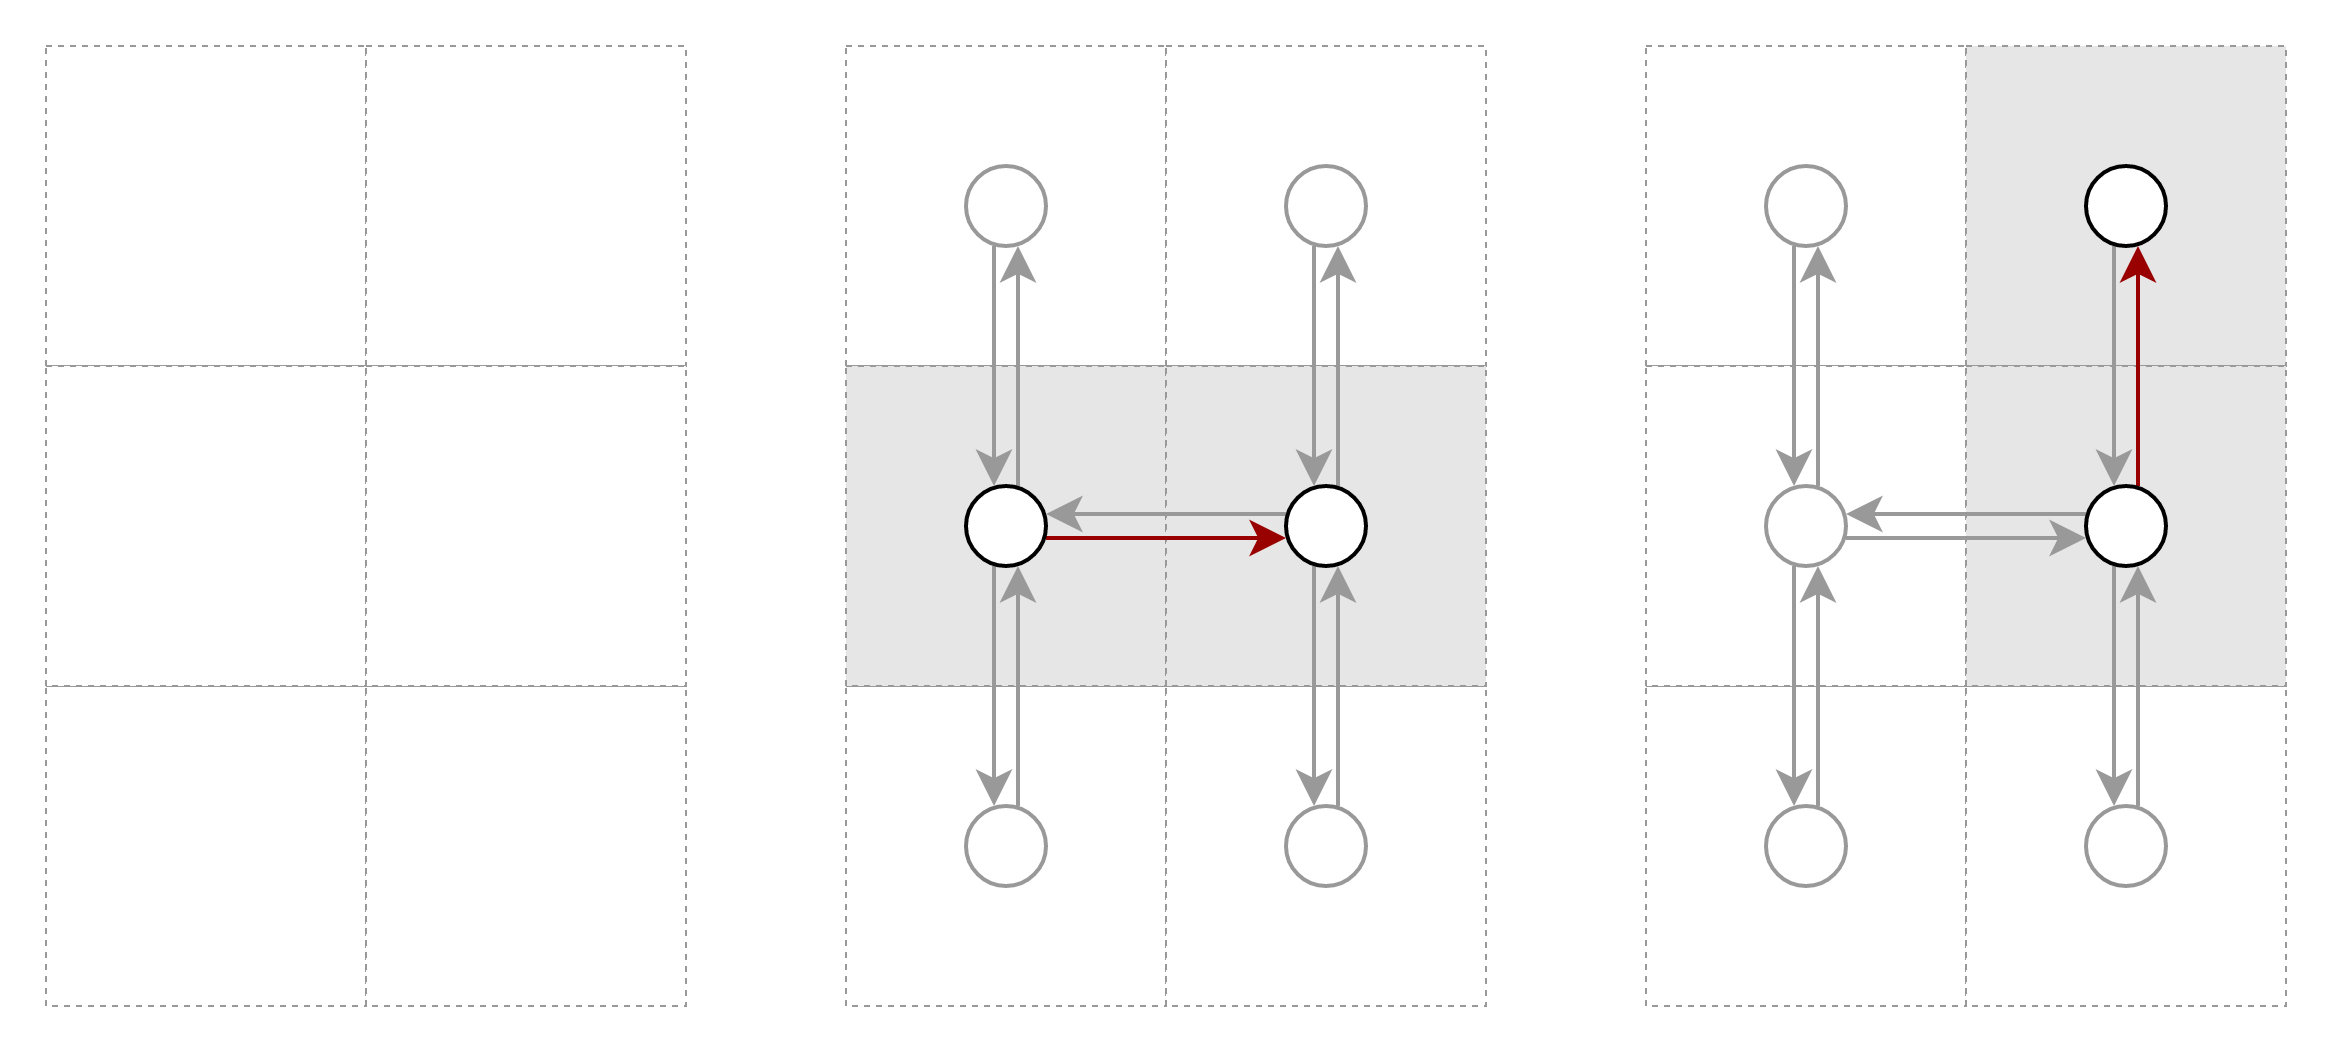
\includegraphics[width=\linewidth]{img/edges.png}
    \caption{Example}
    \label{fig:verticalcell}
\end{figure}

\begin{itemize}
	\item $(n_3 \rightarrow n_4, \{north\}, east)$
	\item $(n_4 \rightarrow n_2, \{north, east\}, north)$
\end{itemize}
